%\documentclass[letterpaper,10pt,twoside,twocolumn,openany]{book}
\documentclass[letterpaper,12pt,openany]{extbook}

\usepackage[francais]{babel}

\usepackage[utf8]{inputenc}

\usepackage{lipsum}
\usepackage{listings}
\usepackage[hidelinks]{hyperref}

\usepackage{float}
\usepackage{dnd}

\usepackage{tikz}
\usetikzlibrary{calc,shadows}

\lstset{%
  basicstyle=\ttfamily,
  language=[LaTeX]{TeX},
}
\setlength{\parindent}{4em}
\setlength{\parskip}{1em}
\renewcommand{\baselinestretch}{1.5}


\newcommand{\md}{·}
\newcommand{\lvlEasy}{facile}
\newcommand{\lvlMedium}{moyen}
\newcommand{\lvlHard}{difficile}

\setlength\parindent{0pt}

% Start document
\begin{document}
\AddToShipoutPicture{\BackgroundPic}

\begin{titlepage} % Suppresses displaying the page number on the title page and the subsequent page counts as page 1
  \raggedleft % Right align the title page

  \rule{1pt}{\textheight} % Vertical line
  \hspace{0.05\textwidth} % Whitespace between the vertical line and title page text
  \parbox[b]{0.75\textwidth}{ % Paragraph box for holding the title page text, adjust the width to move the title page left or right on the page

    {\color{titlered}\Huge\bfseries Manuel de désamorçage}\\[2\baselineskip] % Title
    {\large\textit{À manier avec précaution}}\\[4\baselineskip] % Subtitle or further description
    {
      \textsc{Charles Paulet \\[0.5\baselineskip]
        Léo Paol \\[0.5\baselineskip]
        Théophile Champion \\[0.5\baselineskip]
        Nicolas-Emmanuel Robert
      }
    }

    \vspace{0.4\textheight} % Whitespace between the title block and the publisher

    {
      Version 1.0\\
      EvilTek -- evil engineers of evil corporation\\
      \noindent \url{https://github.com/valkheim/KTNE-IRL}
    }
  }
\end{titlepage}


\renewcommand{\contentsname}{Contenu du manuel}
\tableofcontents

\chapter{Soyez le ou la bienvenu·e}
Pas de chance, vous voici avec la vie de votre ami\md e entre les mains. Ce sont
des choses qui arrivent me direz-vous. Quand bien même on ne l'aurait pas
souhaité c'est un juste retour des choses pour vous de vous retrouver dans cette
situation. Ca vous apprendra à aller fouiller le laboratoire de la société du
mal des ingénieur\md e\md s maléfiques\dots  Maintenant il vous reste à faire de
votre mieux pour ne pas que tout parte en fumée ! Vous trouverez dans ce manuel
toutes les informations (et sûrement beaucoup plus, voire même un peu trop) qui
vous permettrons de désamorçer la bombe, même des plus terribles. Ne négligez
aucun détail, ce serait dommage\dots Mais surtout bonne chance !\par

\section{Petit cours de désamorçage}
Une bombe explose quand le compteur tombe à 00:00. La seule option pour la
désamorcer est de désamorcer chacun de ses modules. Et ils sont nombreux.
Vous devriez pouvoir les discerner, ils sont imbriqués dans la malette.
\subsection{Modules}
Chaque bombe contient onze modules qui doivent être désamorcés. Ils peuvent être
désamorcés dans l'ordre souhaité et normalement ils ne s'influcent pas les uns
les autres. Mais qui sait ce qui se passe dans la tête d'ingénieur\md e\md s
fous\dots Enfin vous verrez bien sur quoi vous tomberez !\par
Dans la suite du manuel vous trouverez les instructions pour désamorcer chacun
des modules. Lisez les instructions attentivement et coordonnez-vous bien avec
votre équipier·ère ou vous n'en ressortiez pas vivant.\par
\subsection{Pénalités}
Eh oui, des pénalités ! Les ingénieur\md e\md s d'EvilTek sont vicieux et se
doutaient bien que des petit\md e\md s rusé\md e\md s comme vous iraient s'amuser
à bidouiller des engins explosifs. C'est pour ça qu'à chaque tentative de
désamorçage infructueuse d'un module, vous subirez des pénalités de temps. Elles
seront d'autant plus importantes que le niveau de difficulté est élevé. Le temps
file mais ne courrez pas plus vite à votre perte, tâchez de réfléchir et de
prendre les bonnes décisions.\par
\subsection{Fouinez}
Les informations ne sont pas forcément là où on les attend. Des numéros, textes,
et dessins disséminés sur la bombe et le manuel pourrait vous être utiles.
Pensez à vérifier l'agencement des modules ou encore votre propre téléphone !
Qui sait ce qu'on pu imaginer les constructeur\md trice\md s\dots

\chapter{Modules}
Les modules peuvent être identifiés à leurs LEDs vertes et rouges qui indiquent
si le module est amorçé ou pas. Le module qui contient l'horloge n'est pas à
désamorçer. Ses LEDs indiquent le désamorçage de la bombe. Au fait, on a
retrouvé une petite note des ingénieurs au labo, vous devriez y jeter un coup
d'oeil :
\vspace{.5cm}
\begin{paperbox}{Note des ingénieurs}
  Avec tous ces fils dans tous les sens, j'espère que ça va pas nous sauter à la
  figure ce machin-chose ! Au pire des cas, le code secret pourra nous faire
  gagner un peu de temps. Jérémy me l'a envoyé la semaine dernière : 413372.
\end{paperbox}
\vspace{.5cm}

Les mots de passe ont heureusement pas l'air très robustes. Nous avons trouvé
les fiches techniques des modules. Ça devrait vous être utile pour enrayer les
méchanismes et vous sauver la vie.
\newpage


\subsection{Patterns}
Des patterns ? Ah ouais ? Ah non des patrons. Quoi ? Des motifs ? Des schémas ?
Décidément, l'anglais technique c'est pas très clair ! Ici il va falloir
reconnaitre des \sout{patrons} motifs et appuyer sur les bons boutons.
\vspace{.5cm}
\begin{modulebox}{Pas terne}
  \begin{hangingpar}
    \begin{flushright}
    \textit{\dots Il fallait que je la fasse celle là}
    \end{flushright}
  \end{hangingpar}
  \modulesection{Description}
  \begin{moduleaction}[Difficulté]
    Pas si facile quand même
  \end{moduleaction}
  \begin{moduleaction}[Table de correspondance]
    \\\hline
    TODO
  \end{moduleaction}
  \hline%
  \modulesection{Composants :}
  \begin{moduleaction}[boutons]
    Il faut les appuyer pour valider un choix. Attention à ne pas se tromper.
  \end{moduleaction}
  \begin{moduleaction}[écran Arduino TFT]
    Un écran LCD rétroéclairé muni d'un emplacement pour carte SD. Avec ça, on
    peut générer tout un tas de formes géométriques et même charger des images.
  \end{moduleaction}
\end{modulebox}
\vspace{.5cm}

Écrire les directives de la résolution du module ici.
\newpage


\subsection{Simon says \dots heu non juste simon}
\lipsum[3]
\newpage

\subsection{Wire Warrior}
Sous ce nom terrible se cacherait-il simplement des fils à brancher, débrancher
et rebrancher correctement ? On l'espère\dots
\vspace{.5cm}
\begin{modulebox}{/wire/warrior -help}
  \begin{hangingpar}
    \textit{Le fil rouge sur le bouton rouge, le fil vert\dots}
  \end{hangingpar}
  \modulesection{Description}
  \begin{moduleaction}[Difficulté]
    Facile
  \end{moduleaction}
  \begin{moduleaction}[Priorités]
    \\\hline
    \begin{dndtable}
      \textbf{difficulté}  & \textbf{levels} \\
      easy      & 1 0 1 \\
      medium    & gnd vcc gnd \\
      hardcore  & 0x00 0x01 0x00 \\
    \end{dndtable}
  \end{moduleaction}
  \hline%
  \modulesection{Composants :}
  \begin{moduleaction}[fils]
    Je comporte pluieurs fils avec tout plein de couleurs.
  \end{moduleaction}
  \begin{moduleaction}[bouton]
    Un bouton de validation pour tester le raccord de fils.
  \end{moduleaction}
  \begin{moduleaction}[résistances]
    Mes résistances de retour sont nécessaire à la bonne lecture des pins.
  \end{moduleaction}
\end{modulebox}
\vspace{.5cm}

Il semblerait que vous devez brancher correctement les fils. Plutôt simple pour
celui-ci. On dit qu'une bonne communication est la clef du succès !
\newpage



\newpage
\begin{tikzpicture}[
    overlay,
    remember picture,
    mynode/.style={left,fill=yellow!10,general shadow={shadow scale=1, shadow xshift=-0.8ex, shadow yshift=-0.8ex, opacity=1, fill=gray!50}},
  ]
  \node[mynode] at ($(current page.north east)+(-0.2,-6)$) {\fontsize{25}{30}\selectfont \textbf{KTNE the IRL version}};
  \node[mynode] at ($(current page.north east)+(-0.5,-8)$) {\fontsize{20}{24}\selectfont \textsc{evil engineers of evil corporation}};
  \node[mynode] at ($(current page.north east)+(-0.8,-10)$) {\fontsize{15}{18}\selectfont EvilTek, 2018};
  \node[above right] at ($(current page.south west)+(2,2)$) {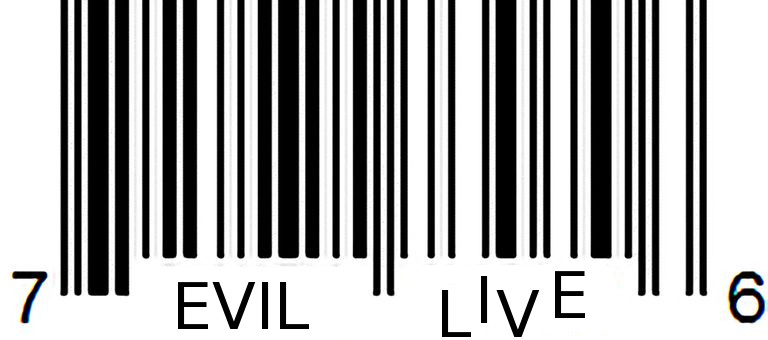
\includegraphics[scale=0.2]{img/barcode}};
\end{tikzpicture}

\end{document}
